\documentclass[french,12pt,a4paper]{article}
\usepackage[T1]{fontenc}
\usepackage[utf8]{inputenc}
\usepackage[dvips]{graphicx}
%\usepackage[english]{babel}
\usepackage[frenchb]{babel}
\AddThinSpaceBeforeFootnotes % à insérer si on utilise \usepackage[french]{babel}
\FrenchFootnotes % à insérer si on utilise \usepackage[french]{babel}
\usepackage{amsmath,amsthm,amsfonts,amssymb}
\usepackage{mathrsfs}
\usepackage{array}
\usepackage{color}
\usepackage{float}
\usepackage{pstricks,pstricks-add,pst-plot,pst-tree}
\usepackage{enumerate}
\usepackage{textcomp}
\usepackage{lscape}
\usepackage{setspace}
\usepackage{lettrine}
\usepackage{lscape}
\usepackage{etex}
\usepackage{lmodern}
\usepackage{stmaryrd}
\usepackage{subfigure}
\usepackage{multido}
\usepackage{listings}
\usepackage{footnote}
\usepackage{appendix}
\usepackage{color}
\usepackage{listings}
\usepackage{tikz}
\usepackage{dsfont}
\usetikzlibrary{matrix}

\lstset{
  language={C++},
  numbers=left, numberstyle=\tiny, stepnumber=1, firstnumber=last,
  frameround=tttt, 
  frame=single, 
  float,
  captionpos=b,
  breaklines=true,
  sensitive=f,
  morestring=[d]",
  basicstyle=\small\ttfamily,
  keywordstyle=\bf\small,
  stringstyle=\sf
}
\usepackage{fancyhdr,lastpage}
\usepackage[twoside,left=2cm,top=2.5cm,dvips,marginparwidth=1.9cm,marginparsep=0.5cm,headheight=35pt]{geometry}
%En tete et pied de page
\usepackage{fancyhdr}
\pagestyle{fancy}
\lhead{\leftmark} 
\chead{}
\rhead{Caclul parallèle avancé	}
\lfoot{ENSIMAG 3A}
\cfoot{\textit{Guillaume Fuchs}}
\rfoot{\thepage}
\renewcommand{\headrulewidth}{0pt}  
\renewcommand{\footrulewidth}{0.4pt}
\title{Calcul parallèle avancé}
\author{Guillaume Fuchs}
%Page de garde

\begin{document}
\begin{titlepage}
\begin{center}

\textsc{\LARGE ENSIMAG}\\[1.5cm]

\textsc{\Large Calcul parallèle avancé}\\[0.5cm]

% Title
 \hrule
 \hrule 

\vspace{7mm}
{ \huge \bfseries Parallélisation du pricer}

\vspace{7mm}
\hrule
\hrule

\vspace{7mm}
% Author and supervisor
\begin{minipage}{0.4\textwidth}
\begin{flushleft} \large
\emph{Etudiant:}\\
Guillaume \textsc{Fuchs}\\
\end{flushleft}
\end{minipage}

\vfill

% Bottom of the page
{\large \today}

\end{center}
\end{titlepage}
\newpage

L'objectif de ce rapport est de montrer les résultats de l'implémentation parallèle sur GPU du pricer Monte-Carlo réalisé durant le cours Modélisation et programmation de 2A. La première partie du document présente la démarche analytique mise en place pour la parallélisation. Enfin, la deuxième partie présentera et étudiera les résultats de performance obtenues avec cette implémentation. 

\section{Conception du pricer sur GPU}

\begin{center}
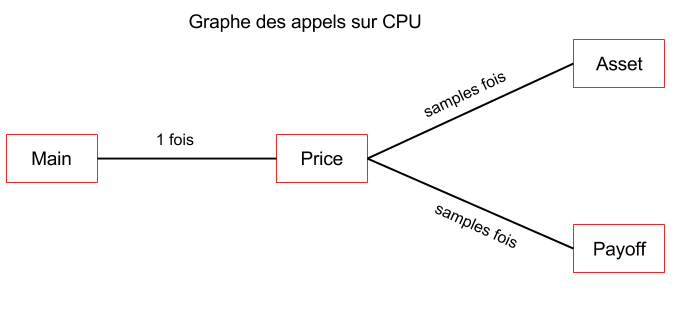
\includegraphics[scale=0.6]{appelCPU.png}
\end{center}

Ce que l'on constate sur le graphe des appels sur CPU c'est que la procédure \lstinline!price! appel un très grand nombre de fois en série les procédures \lstinline!asset! et \lstinline!payoff!. Il semble donc important de pouvoir paralléliser ces deux procédures afin de réaliser les différents appels.\\

Le pricer sur GPU alloue des blocs de dimension \textit{1*512} et une grille dont le nombre de blocs dépend du nombre de samples. On subdivise le nombre de samples en un nombre optimal de samples (\textit{OptimalSamples}) selon la taille et le nombre de pas de temps de l'option. Il va correspondre au nombre de thread total qui calculeront une estimation du prix de l'option. On défini ce nombre de samples par: 
$$OptimalSamples = \frac{10 240}{N*size}$$

Le nombre $10 240$ est déterminé par des tests de performance sur différentes options que nous verrons plus tard et dépend aussi de la machine sur laquelle les tests sont effectués.\\

Le pricer va posséder une boucle principal qui va calculer le prix et l'intervalle de confiance d'une option possédant un nombre de samples égal à $OptimalSamples$. La somme de ces prix et de ces intervalles sur la boucle complète va nous donner le prix et l'intervalle de confiance demandé (avec le nombre de samples total).\\
Avant d'entrer dans la boucle, la fonction appel \lstinline!init_rand! (fonction sur GPU) qui va permettre d'initialiser la graine du générateur de nombre aléatoire. Le nombre de thread total qui vont l'appeler sur un tour de boucle est de $OptimalSamples*N*size$.\\
Sur un tour de boucle les appels sont:
\begin{itemize}
	\item \lstinline!make_rand! (fonction sur GPU) qui va permettre d'associer à chaque thread un nombre aléatoire issue de la loi normale centrée réduite. Le nombre de thread total qui vont l'appeler est de $OptimalSamples*N*size$.
	\item \lstinline!assetGPU! (fonction sur CPU) qui va permettre de générer l'ensemble des chemins de l'option en utilisant \lstinline!asset_compute! (fonction sur GPU). A noter que le nombre de thread total qui vont appeler cette fonction est différent du nombre de thread total dans \lstinline!make_rand! et \lstinline!init_rand! car dans \lstinline!assetGPU!, un thread va créer $size$ chemins de $N$ pas de temps ce qui correspond à une option. Il utilisera donc les $size * N - 1$ threads suivant pour obtenir une suite d'échantillon de loi normale centrée réduite indépendante et identiquement distribuée. Le nombre de thread total qui appellerons la fonction est de $OptimalSamples$.
	\item \lstinline!price_mc! qui va appeler selon le type de l'option la fonction associée pour permettre de calculer le prix et l'intervalle de confiance sur un nombre de samples donné par une méthode de réduction par \lstinline!mc_option! (fonction sur GPU). Le nombre de thread total qui appellerons la fonction est de $OptimalSamples$.
\end{itemize}

Le graphe des appels sur CPU/GPU est donc le suivant:

\begin{center}
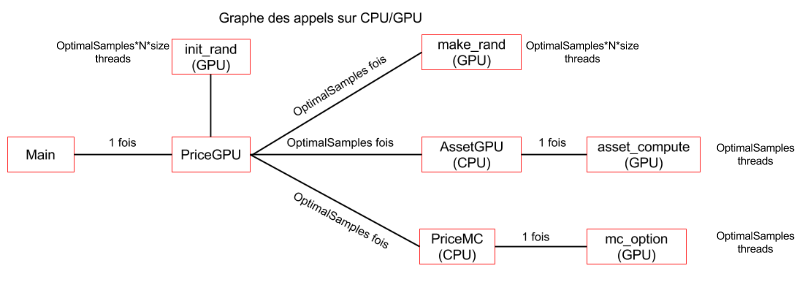
\includegraphics[scale=0.5]{appelGPU.png}
\end{center}

\section{Analyse des performances}

Les tests de performance ont été effectués sur une carte graphique NVIDIA GeForce GT 750M. Les informations obtenus via \lstinline!cudaGetDevicePropertiesl! sont:
\begin{itemize}
	\item Taille mémoire globale 4 294 967 295
	\item Taille mémoire constante: 65 536
	\item Taille mémoire partagée: 49 152
	\item Nombre de threads maximum par direction: 1024 x 1024 x 64
	\item Nombre maximum de thread par bloc: 1024
	\item Nombre de blocs par grille: 2 147 483 647 x 65 535 x 65 535
\end{itemize}

\subsection{Détermination du nombre samples optimal}

Pour déterminer le nombre de samples optimal qui va correspondre à calculer pour chaque tour de boucle une option possédant un nombre de samples égal à $OptimalSamples$, on détermine le temps d'exécution de différentes options (ici "call", "asian0", "barrier") en fonction du nombre $x$ qui est présent dans $\frac{x}{N*size}$. \\

\begin{center}
\begin{figure}
   \begin{minipage}[c]{.46\linewidth}
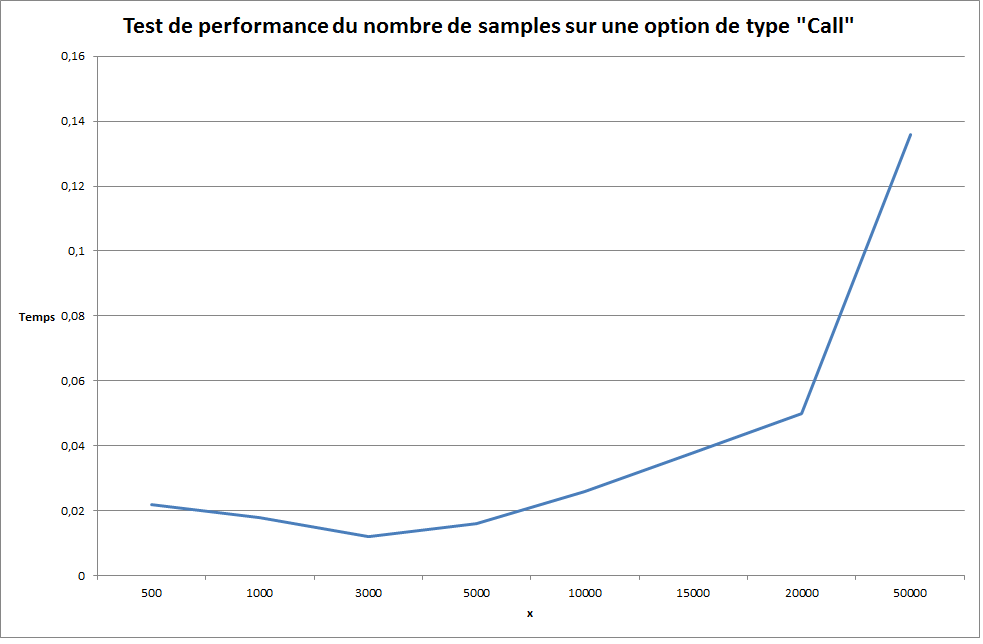
\includegraphics[scale=0.3]{samples_call.png}
   \end{minipage} \hfill
   \begin{minipage}[c]{.46\linewidth}
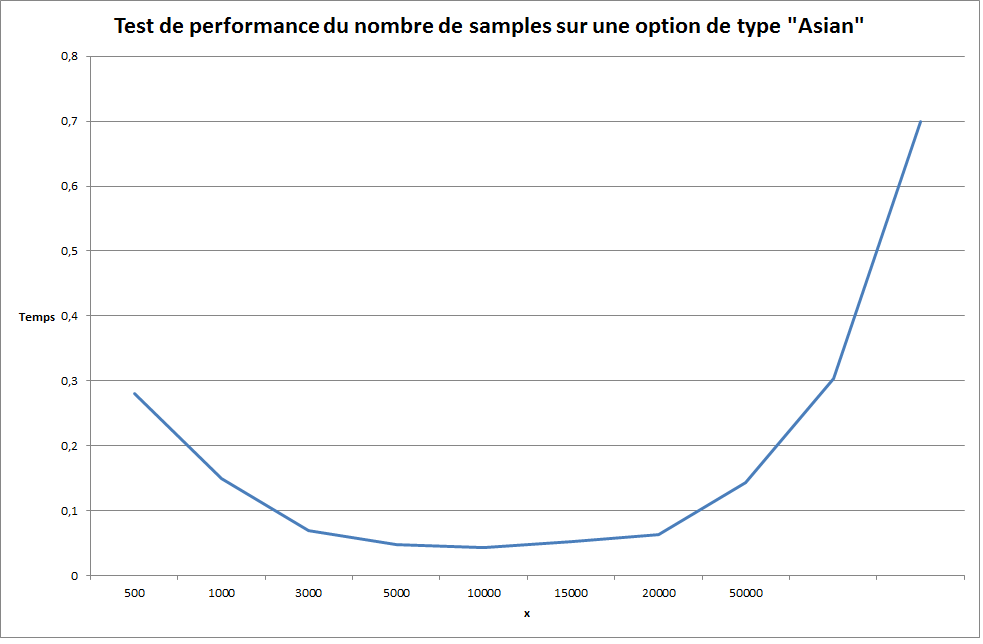
\includegraphics[scale=0.3]{samples_asian.png}
   \end{minipage}
\end{figure}
\begin{figure}

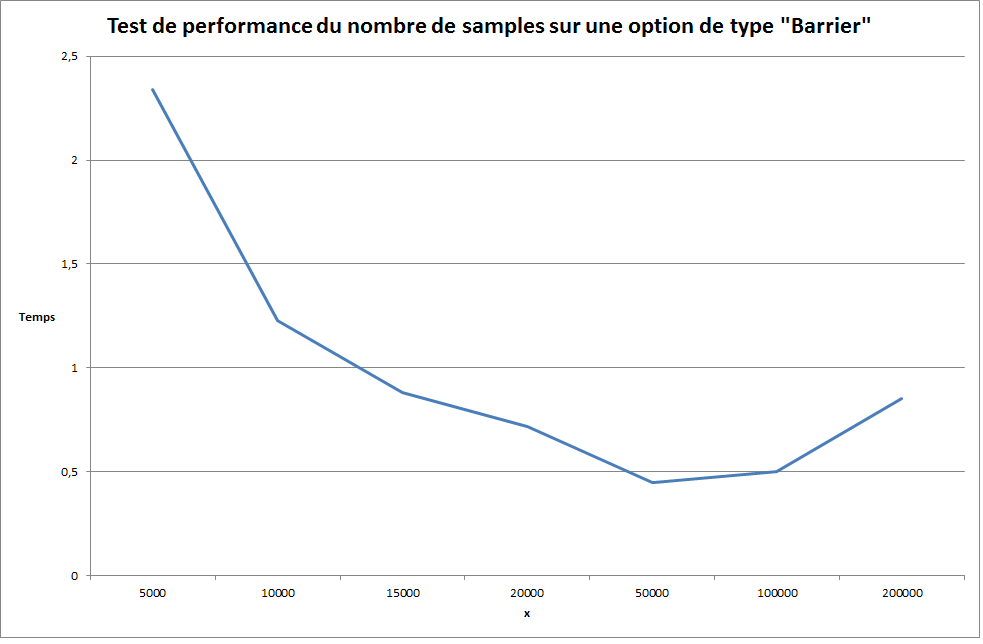
\includegraphics[scale=0.3]{samples_barrier.png}

\end{figure}
\end{center}


Ces tests de temps d'exécution montre que selon le type de l'option, le nombre de samples optimale est différent. Les options de type "Call" ne demandent pas de parcourir les N prix du sous-jacent contrairement aux options de type "Asian" et "Barrier". Chaque thread ne passe pas beaucoup de temps dans le calcul du premier type d'option tandis que dans le deuxième type d'option, les threads passent beaucoup de temps pour calculer un prix. \\

Dans le cas du pricer, nous avons fixé le nombre $x$ à $10 240$ pour ne contraindre aucun type d'option sachant que les options de type "Call" ne demandent que très peu de temps de calcul.\\
Il serait intéressant de continuer cette étude sur le temps d'exécution par rapport au nombre de samples optimal afin pouvoir modifier le nombre optimal de samples selon le type d'option.\\

\newpage
\subsection{Test de performance}
 On s'intéresse ici à l'évolution du temps d'exécution du pricer sur deux type d'option: une option "call" et une option "barrier". De plus, on compare le temps d'exécution avec le pricer conçut en 2A qui s'exécute uniquement sur CPU.\\
 
\begin{center}
\begin{figure}[h!]

   \begin{minipage}[c]{.46\linewidth}
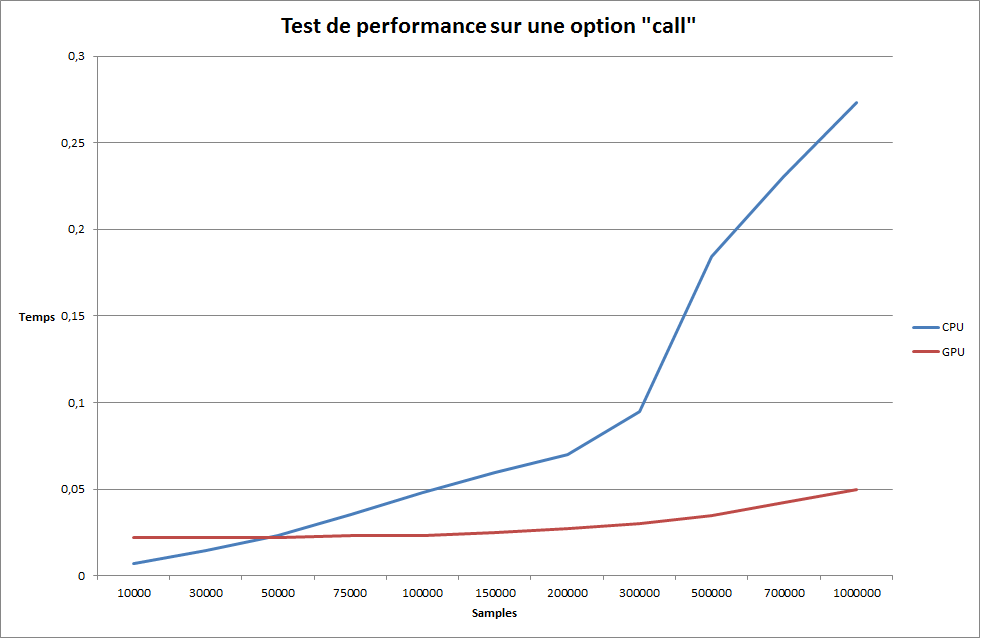
\includegraphics[scale=0.3]{call.png}
   \end{minipage} \hfill
   \begin{minipage}[c]{.46\linewidth}
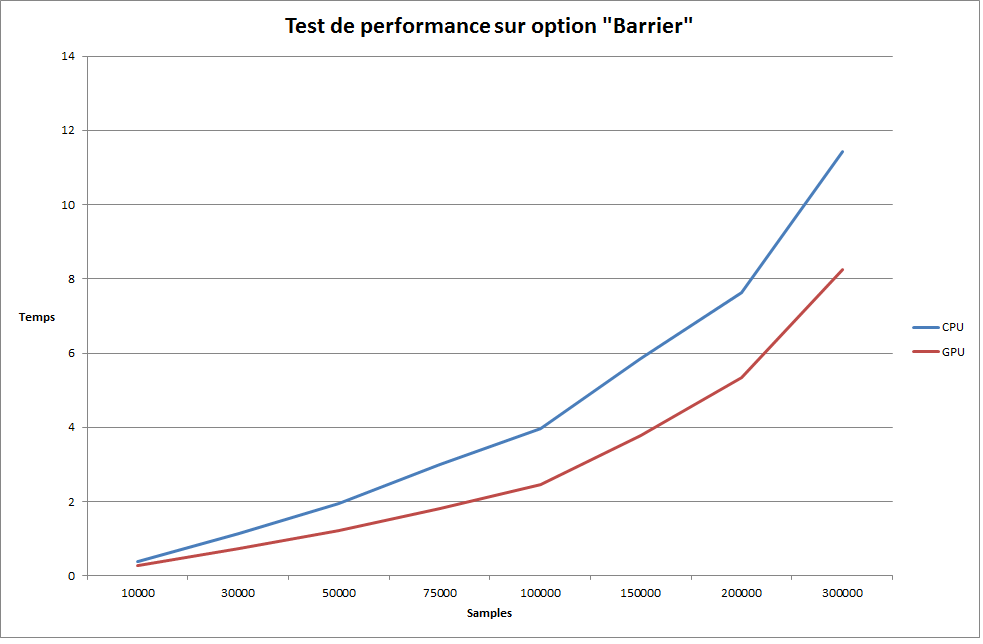
\includegraphics[scale=0.3]{barrier.png}
   \end{minipage}
\end{figure}
\end{center}

On constate que pour une option de type "call", le temps d'exécution augmenter de façon linéaire sur CPU/GPU tandis qu'il augmente de façon exponentielle sur CPU. En effet à partir de 300 000 échantillons, le temps d'exécution du pricer sur CPU augmente de façon très forte. Cela peut s'expliqué par le fait que la mémoire utilisé pour le pricer sur CPU/GPU est constante (on utilise toujours une taille de mémoire qui est proportionnel à $OptimalSamples$ et qui est constante quelle que soit le nombre de samples total), tandis que sur CPU, on alloue des tableaux de taille $Samples$ qui correspond au nombre total d'échantillon. Si ce nombre augmente, la mémoire peut saturer et les calculs sont plus lent à effectuer.\\
De plus, pour un nombre d'échantillon faible (de l'ordre de 10 000), le temps  d'exécution sur CPU est plus faible que le temps d'exécution sur CPU/GPU. Ce temps est du au fait que la mémoire à utiliser est très faible sur CPU et que les calculs se font très rapidement car la mémoire n'affecte pas le temps d'exécution. Sur CPU/GPU, la mémoire utilisée est constante et peut être plus élevée que sur CPU.\\

Sur une option de type "barrier", le temps d'exécution augmente de la même façon que l'on soit sur CPU ou sur CPU/GPU avec un temps d'exécution toujours plus faible pour le pricer sur CPU/GPU. L'option de type "barrier" demande lors du calcul du payoff de parcourir l'esnemble des prix du sous-jacent sur la durée de vie de l'option. Le fait de pouvoir parcourir de façon parallèle plusieurs chemins permet d'obtenir un gain de temps par rapport à parcourir de façon séquentielle les chemins.
\end{document}
